% !TEX root = ../../Main.tex
\section{Results Across the Seven Majors}
\label{Section:PairResults}

\Cref{Tables:PairResults} gives the result for each pair, in alphabetical order. Total return over the eleven years goes from $+226.6\%$ on USD/CAD, the highest, to $+15.7\%$ on USD/JPY, the lowest. Every pair is profitable, and every pair is profitable from all five starting balances.

% !TEX root = ../Main.tex
\begin{table}[htb!]
\centering
\footnotesize
\caption{Result for each pair from 2015 to 2026. The return columns give the mean, standard deviation and range across the five starting balances of \Cref{Section:EvaluationProtocol}. Every pair is profitable from all five. Ratios and drawdown are from the reference run. USD/CAD returns the most, and USD/CHF is best on every risk measure.}
\label{Tables:PairResults}
\begin{tabular}{@{}lrrrrrrrrr@{}}
\toprule
\textbf{Pair} & \textbf{Mean} & \textbf{SD} & \textbf{Min} & \textbf{Max} & \textbf{Sharpe} & \textbf{Sortino} & \textbf{Calmar} & \textbf{Max DD} & \textbf{Trades} \\
\midrule
AUD/USD & 102.5\% & 10.6 & 87.2\% & 117.1\% & 0.348 & 0.496 & 0.143 & 41.1\% & 1,561 \\
EUR/USD & 73.9\% & 3.3 & 69.5\% & 77.8\% & 0.387 & 0.544 & 0.106 & 46.8\% & 1,778 \\
GBP/USD & 124.1\% & 5.1 & 115.1\% & 129.1\% & 0.397 & 0.563 & 0.155 & 50.4\% & 2,516 \\
NZD/USD & 56.4\% & 3.8 & 52.2\% & 61.7\% & 0.368 & 0.531 & 0.187 & 23.3\% & 1,011 \\
USD/CAD & \textbf{226.6\%} & 10.8 & 216.9\% & 246.0\% & 0.603 & 0.870 & 0.228 & 49.1\% & 2,213 \\
USD/CHF & 50.6\% & 5.2 & 43.4\% & 56.4\% & \textbf{0.802} & \textbf{1.552} & \textbf{0.492} & \textbf{8.2\%} & 220 \\
USD/JPY & 15.7\% & 0.7 & 14.5\% & 16.5\% & 0.251 & 0.342 & 0.057 & 24.0\% & 1,438 \\
\bottomrule
\end{tabular}
\end{table}

One fact is important for everything that follows, and it is easy to miss. \textbf{Five of the seven pairs lost value over the eleven years.} A trader who had simply bought and held would have finished down $26.1\%$ on NZD/USD, $20.3\%$ on USD/CHF, $18.2\%$ on AUD/USD, $13.5\%$ on GBP/USD and $2.9\%$ on EUR/USD. Only USD/CAD, at $+18.1\%$, and USD/JPY, at $+30.7\%$, rose. The agents made money on all seven. On five of them, the return was therefore earned in a falling market, and not in a rising one.

% !TEX root = ../Main.tex
\begin{table}[htb!]
\centering
\footnotesize
\caption{Each agent against buying and holding its own pair over the same window and under the same costs. Five of the seven pairs lost value over the eleven years, so on those the return was earned against a falling market. USD/JPY is the only pair whose benchmark rose substantially, and the only one the agent failed to beat.}
\label{Tables:Benchmark}
\begin{tabular}{@{}lrrrr@{}}
\toprule
\textbf{Pair} & \textbf{Market} & \textbf{Model} & \textbf{Excess} & \textbf{Positive Years} \\
\midrule
AUD/USD & $-18.2\%$ & $+87.2\%$ & $+105.4$ pp & 8 of 11 \\
EUR/USD & $-2.9\%$ & $+70.6\%$ & $+73.4$ pp & 5 of 11 \\
GBP/USD & $-13.5\%$ & $+129.1\%$ & $+142.5$ pp & 7 of 11 \\
NZD/USD & $-26.1\%$ & $+60.1\%$ & $+86.1$ pp & 7 of 11 \\
USD/CAD & $+18.1\%$ & $+221.0\%$ & $+202.9$ pp & 8 of 11 \\
USD/CHF & $-20.3\%$ & $+54.8\%$ & $+75.2$ pp & \textbf{10 of 11} \\
USD/JPY & $+30.7\%$ & $+16.2\%$ & $\mathbf{-14.4}$ pp & 5 of 11 \\
\bottomrule
\end{tabular}
\end{table}

The rest of this section discusses each pair in turn, in alphabetical order. For each pair it covers what the market did, what the agent returned in comparison, how that return decomposes into policy and market exposure, what the agent paid in costs, and how it traded.

\subsection{AUD/USD}

The Australian Dollar fell $18.2\%$ against the US Dollar over the eleven years. The agent returned $+87.2\%$, which is $105.4$ percentage points above holding the pair. It earned this from the short side: only $27.9\%$ of its $1\,561$ positions were long.

This result needs care in the alpha and beta decomposition. Its beta of $-2.013$ is the largest negative beta of the seven. This means that the agent was short the falling market at roughly twice its size. Of its $8.18\%$ mean yearly return, $4.96$ points are alpha and $3.22$ points are beta return, from the general fall of the market. Close to two fifths of what it earned therefore came from the Australian Dollar falling, and not from choosing when to be short. The policy does make a profit, but part of that profit would turn into a loss in a decade where the pair rose.

It trades at a moderate pace. Its median holding period is $9.7$ days, its average size is $0.77$ of the reference size, and its win rate is $52.7\%$. It made $10\,689$ euros of gross profit and paid $2\,200$ in commission. That is a $20.6\%$ share, the highest of the seven, and it comes directly from its turnover. The equity curve is uneven. Eight of eleven years are positive. The best year is 2024, at $+72.4\%$ and $81.6$ points above the benchmark, and the worst is 2017, at $-22.5\%$. Its maximum drawdown is $41.1\%$.

\begin{figure}[htb!]
\centering
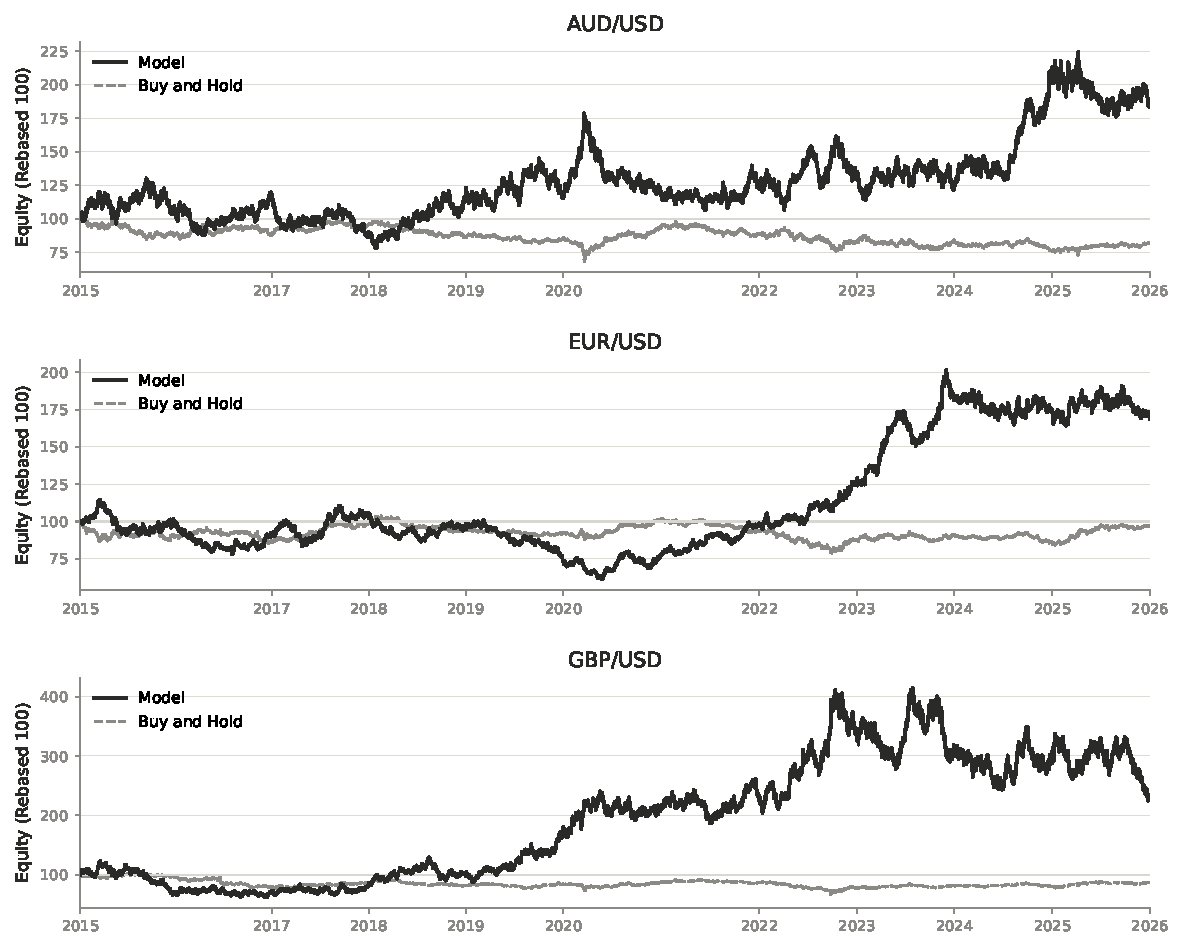
\includegraphics[width=\textwidth]{Images/PairEquityA.pdf}
\caption{AUD/USD, EUR/USD and GBP/USD against buying and holding the same pair, rebased to 100. All three benchmarks finish below their starting level.}
\label{Figure:PairEquityA}
\end{figure}

\subsection{EUR/USD}

EUR/USD is the clearest example in this work of a return that does not come from market exposure. The pair finished almost exactly where it started, down $2.9\%$ over eleven years, and the agent returned $+70.6\%$. Its beta is $+0.266$, and market exposure adds $0.01$ percentage points per year. Of a $6.63\%$ mean yearly return, $6.62$ points are therefore attributable to the policy. The market had no trend for the agent to follow, so the return came from timing alone.

It has the shortest holding period of the seven, a median of $3.9$ days, and it trades at a low $0.40$ of the reference size. Its exposure is close to balanced, with $55.5\%$ long across $1\,778$ positions. It won $51.9\%$ of them. Gross profit of $8\,734$ euros became $7\,064$ after $1\,669$ euros of commission, a $19.1\%$ share.

The equity curve in \Cref{Figure:PairEquityA} shows that the headline return also needs care here, for a different reason than on AUD/USD. Only five of eleven years are positive. The agent is roughly flat for the first six years of the window. It makes almost all of its return between 2021 and 2023, when the pair moved in unusually wide ranges: $+27.3\%$, $+29.0\%$ and $+44.0\%$ in those three years, against $-25.3\%$ in 2019. This policy needs volatility to work. Its maximum drawdown of $46.8\%$ comes from the periods when there was not enough volatility.

\subsection{GBP/USD}

GBP/USD has the highest alpha of the seven, at $+11.64\%$ per year, with a beta of $-0.054$ that is statistically indistinguishable from zero. Its mean yearly return is $11.70\%$, and only $0.06$ points of it come from market exposure. It is as close to pure policy as any result in this chapter. Sterling itself fell $13.5\%$ over the window, so the agent's $+129.1\%$ is $142.5$ percentage points above the benchmark.

It is the most active model, with $2\,516$ positions. It also holds them the longest of the six working agents, with a median of $12.6$ days. It therefore keeps many positions open at the same time, and does not trade quickly. It trades near full size, at $0.89$, and wins $51.3\%$ of the time. Gross profit was $16\,630$ euros against $3\,168$ of commission, which left $13\,462$.

Its returns come mostly from the years when sterling moved sharply. These show in \Cref{Figure:PairEquityA} as two steep sections: $+82.2\%$ in 2019 and $+52.0\%$ in 2022. \Cref{Section:TradingBehaviour} looks at the second of these in detail. The same aggressive trading also produces the worst single year of any agent, $-31.6\%$ in 2015, and the deepest drawdown, $50.4\%$. Seven of eleven years are positive. This is the most volatile of the profitable models. A reader should weigh its alpha against a drawdown that halved the account.

\subsection{NZD/USD}

The New Zealand Dollar fell the most of the seven, $26.1\%$ over the window. The agent returned $+60.1\%$, an excess return of $86.1$ points over the benchmark. Like AUD/USD, it traded mostly from the short side, with $24.0\%$ of positions long and a beta of $-0.708$.

Its alpha of $+2.79\%$ per year is the smallest of the six profitable models. Of its $4.62\%$ mean return, $1.83$ points are beta return. A large part of what it earned, though less than half, therefore came from the market falling and not from timing. By alpha and beta, it is the weakest of the six that worked.

\Cref{Figure:PairEquityB} shows it next to USD/CAD and USD/CHF. This agent is careful, and its risk numbers show the benefit. It takes the fewest positions of the active models, $1\,011$, and holds an average of $0.24$ of the reference size. Its maximum drawdown is $23.3\%$, the second lowest of the seven. Its Calmar ratio of $0.187$ is better than that of four pairs that returned much more. This shows why return is measured against drawdown, and not on its own. Gross profit was $7\,314$ euros and commission $1\,424$, a $19.5\%$ share. Seven of eleven years are positive. The best is 2022 at $+14.5\%$ and the worst is 2016 at $-6.4\%$. It is the steadiest of the models of moderate size.

\begin{figure}[htb!]
\centering
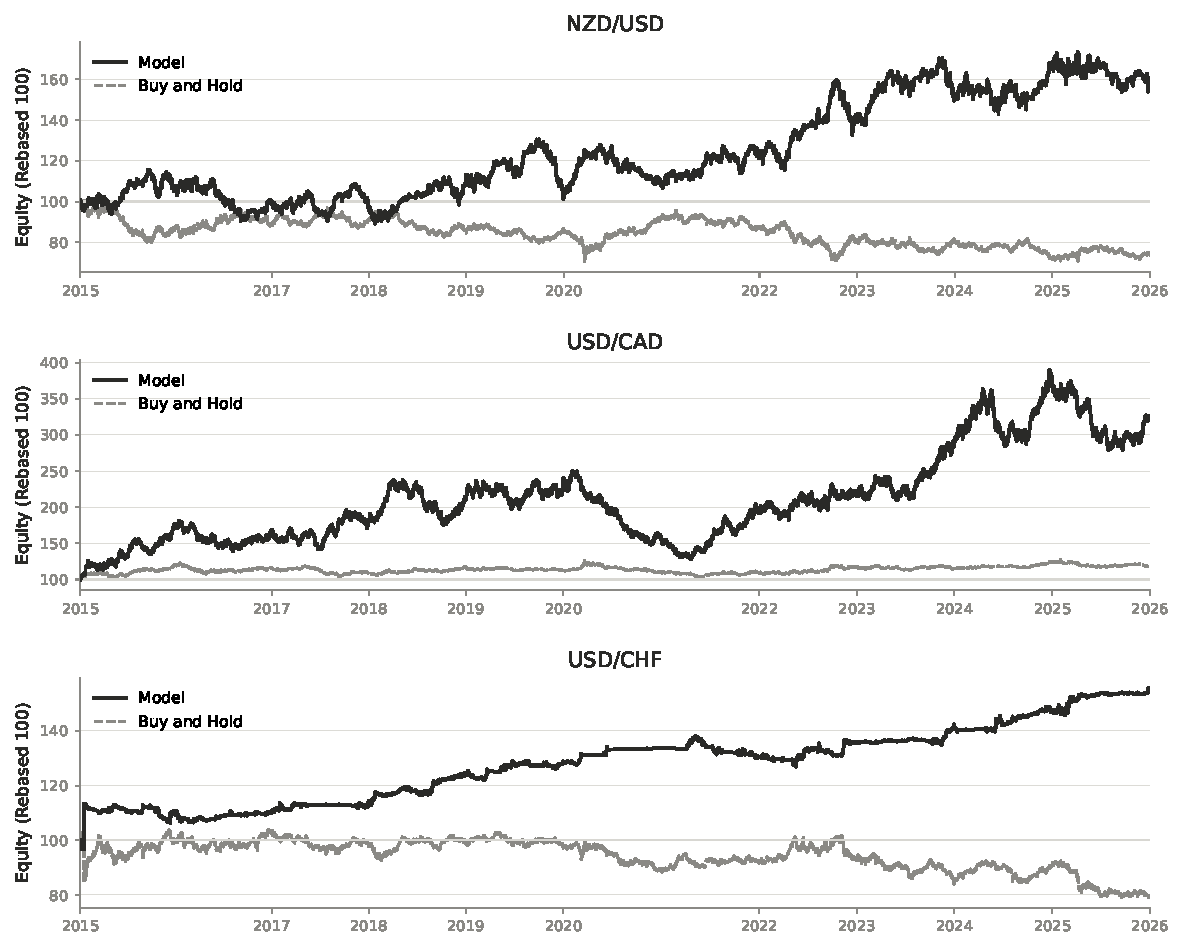
\includegraphics[width=\textwidth]{Images/PairEquityB.pdf}
\caption{NZD/USD, USD/CAD and USD/CHF against buying and holding the same pair, rebased to 100. USD/CAD is the only one of the three whose benchmark rises.}
\label{Figure:PairEquityB}
\end{figure}

\subsection{USD/CAD}

USD/CAD returned $+226.6\%$, by far the largest total in this work. It is also the result that must be read most carefully. Its beta of $+2.393$ is the highest of the seven, and the pair itself rose $18.1\%$. The agent was therefore long a rising market at more than twice its size. Of a $14.23\%$ mean yearly return, $4.21$ points are beta return and $10.02$ are alpha.

That alpha is real, and it is the second highest of the seven. So the model does not look good only because its market went up. But leverage is symmetric: it raises losses as much as gains, and the yearly record shows both. The best year is 2015, at $+71.7\%$ and $52.7$ points above the benchmark. The worst is 2020, at $-34.8\%$. Its maximum drawdown is $49.1\%$, and recovering from a $49\%$ drawdown needs a $96\%$ gain. Eight of eleven years are positive.

It is the second most active model, with $2\,213$ positions and a median holding period of $5.7$ days. It trades at $0.79$ of the reference size and has the highest win rate of the seven, at $55.0\%$. It also earned the most in euros, $25\,577$ gross, and paid $3\,432$ in commission. That is a $13.4\%$ share, lower than for the four pairs discussed above, because its profit per position was larger.

\subsection{USD/CHF}

USD/CHF returned $+54.8\%$. It is fifth of seven on return and first on every risk-adjusted measure. Its Sharpe ratio of $0.802$, Sortino ratio of $1.552$ and Calmar ratio of $0.492$ are the highest of the seven. Its maximum drawdown of $8.2\%$ is a sixth of the worst. The Swiss Franc strengthened over the period, so the pair fell $20.3\%$. With a beta of $-0.082$, the agent took almost none of that movement: of a $4.07\%$ mean yearly return, $3.91$ points are alpha.

Its trading explains all of these numbers. It takes $220$ positions in eleven years, roughly one every eighteen days. It holds an average of $0.09$ of its reference size, a tenth of what it is allowed. Because it trades so little, it pays almost nothing to trade: $130$ euros of commission against $5\,587$ of gross profit. That is a $2.3\%$ share, where the average of the seven is $16.0\%$. It keeps $97.7\%$ of what it earns, while AUD/USD keeps $79.4\%$.

It is positive in ten of eleven years, the most consistent record in this work, and its worst year is $-2.4\%$. Its win rate of $49.8\%$ is the lowest of the seven. This point deserves attention. The best model of the seven is wrong slightly more often than a coin toss. It is still the best because of how it sizes and holds the positions it gets right. It is also the only model that made money in the held-out year of \Cref{Section:OutOfSample}. On return alone it would have placed fifth and would not have been chosen. The selection criteria of \Cref{Section:ExperimentalProcedure} are there to prevent this.

\subsection{USD/JPY}

USD/JPY is the one failure of the seven, and it is the only pair whose benchmark rose by a large amount. The pair gained $30.7\%$ over the window, while the agent returned $+15.7\%$. It finished $14.4$ percentage points behind an investor who bought the pair and did nothing. Its beta of $+1.012$ and its correlation of $+0.946$ with the pair's own yearly move show what it became: a plain long position in the pair, with extra trading and extra costs. Its alpha is $-1.08\%$ per year, the only negative figure in \Cref{Tables:AlphaBeta}.

Every position it takes is long. Its median holding period is measured in years, not days. Its average action is $0.98$. This means it holds almost full size all the time and no longer makes a sizing decision at all. It earned $1\,761$ euros gross, the least of the seven, and paid $155$ in commission. Five of eleven years are positive.

\begin{figure}[htb!]
\centering
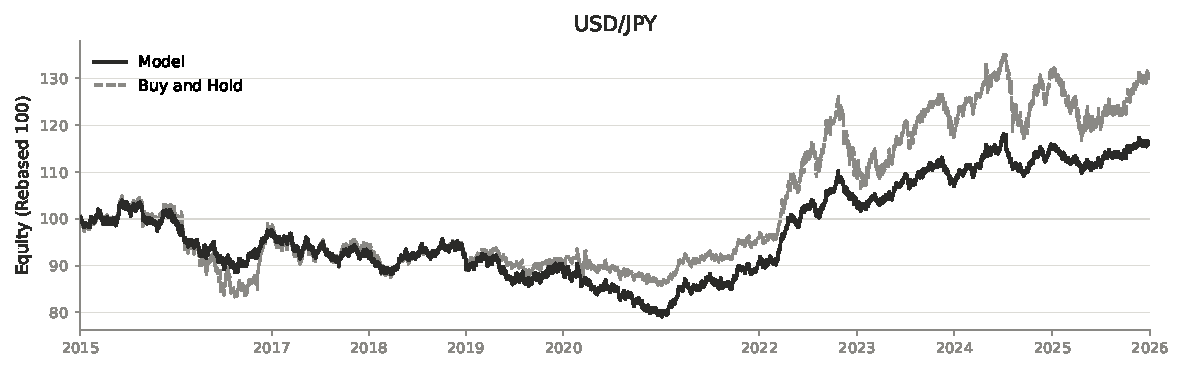
\includegraphics[width=\textwidth]{Images/PairEquityC.pdf}
\caption{USD/JPY against buying and holding the pair. The two lines move closely together. This is what a beta of $+1.012$ looks like, and it is the reason this result is reported as a failure.}
\label{Figure:PairEquityC}
\end{figure}

\Cref{Figure:PairEquityC} shows this more clearly than the statistics do: the model and the benchmark move together, with the model slightly below. \Cref{Section:NegativeResult} explains the cause and what was tried to fix it.